\subsection*{ГЛ13 4}
\begin{figure}[h!]
	\center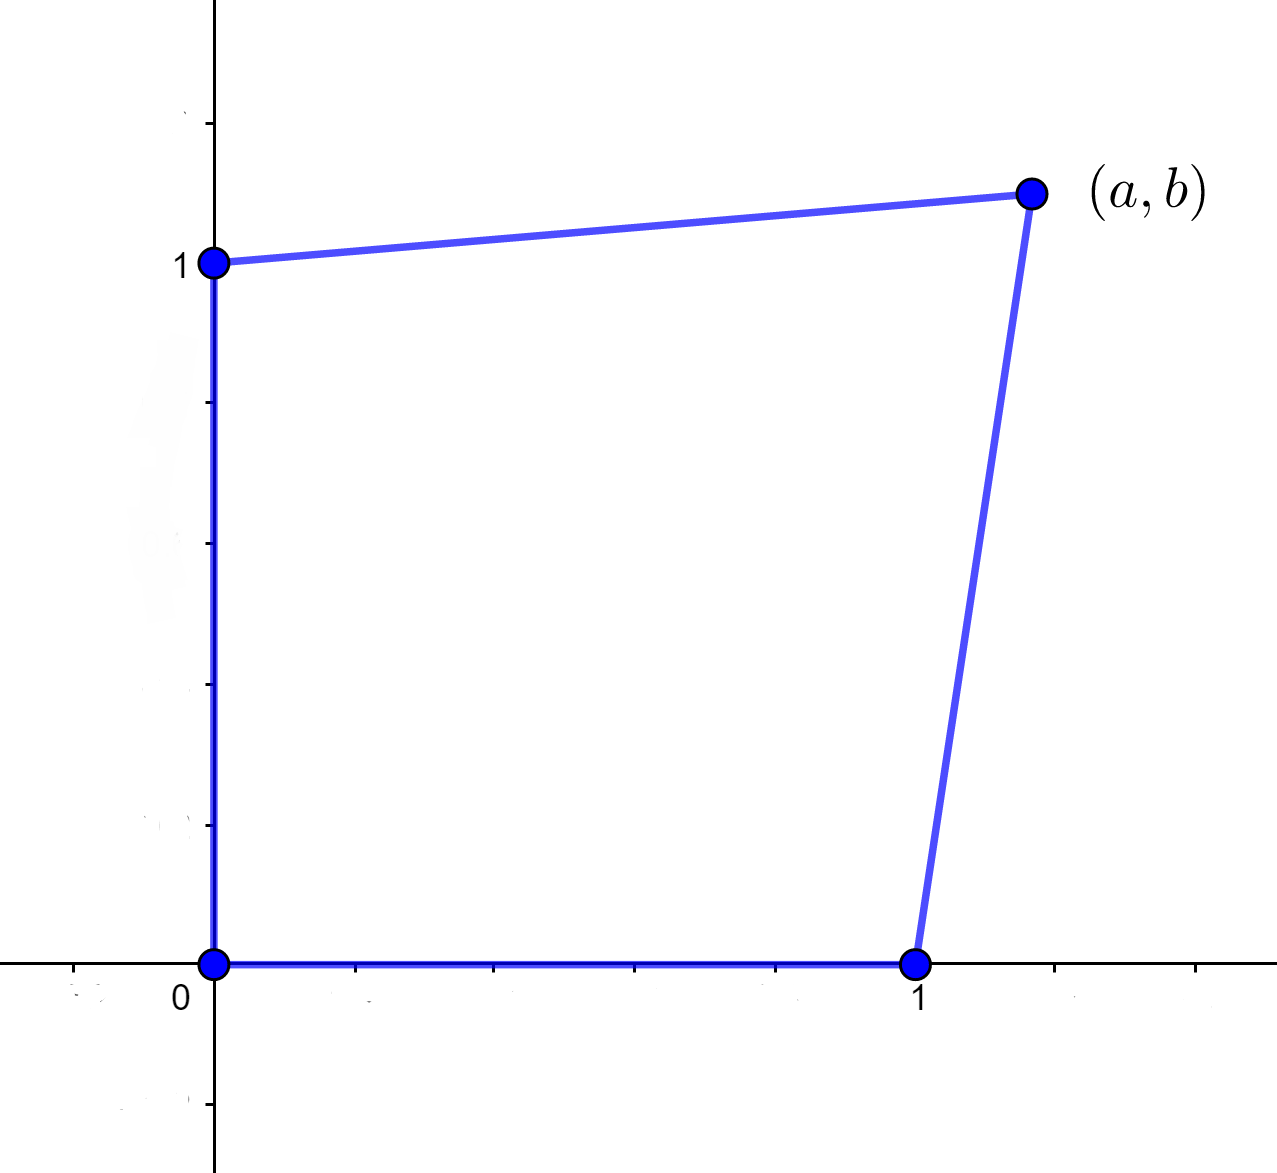
\includegraphics[width=0.35\linewidth]{pic22}
\end{figure}
\noindent
Рассмотрим пучок коник через точки $A_1 = (0,0),\ A_2 = (1,0),\ A_3 = (0,1),\ A_4 = (a,b)$, где $a,b > 0,\ a+b > 1$\\
\begin{gather*}
	C_1: x(x-a) = f(x,y)\\
	C_2: y(y-b) = g(x,y)
\end{gather*}
Пусть пятая точка имеет координаты $A_5 = (c,d)$\\
\begin{gather*}
	C_{A_5} f(A_5) g(A) - g(A_5) f(A) = x(x-a) d(d-b) - y(y-b) c(c-a)
\end{gather*}
Будем считать, что это было в карте $Z = 1$
\begin{gather*}
	\begin{pmatrix}
		0 & \ldots & \ldots\\
		\vdots & d(d-b) & 0\\
		\vdots & 0 & -c(c-a)
	\end{pmatrix}\\
	\\
	\text{det}
	\begin{pmatrix}
	d(d-b) & 0\\
	0 & -c(c-a)
	\end{pmatrix}
	=
	-d(d-b)c(c-a) = A
\end{gather*}
$A > 0$, если $d(d-b)c(c-a) < 0$, в этом случае коника -- эллипс
\begin{figure}[h!]
	\center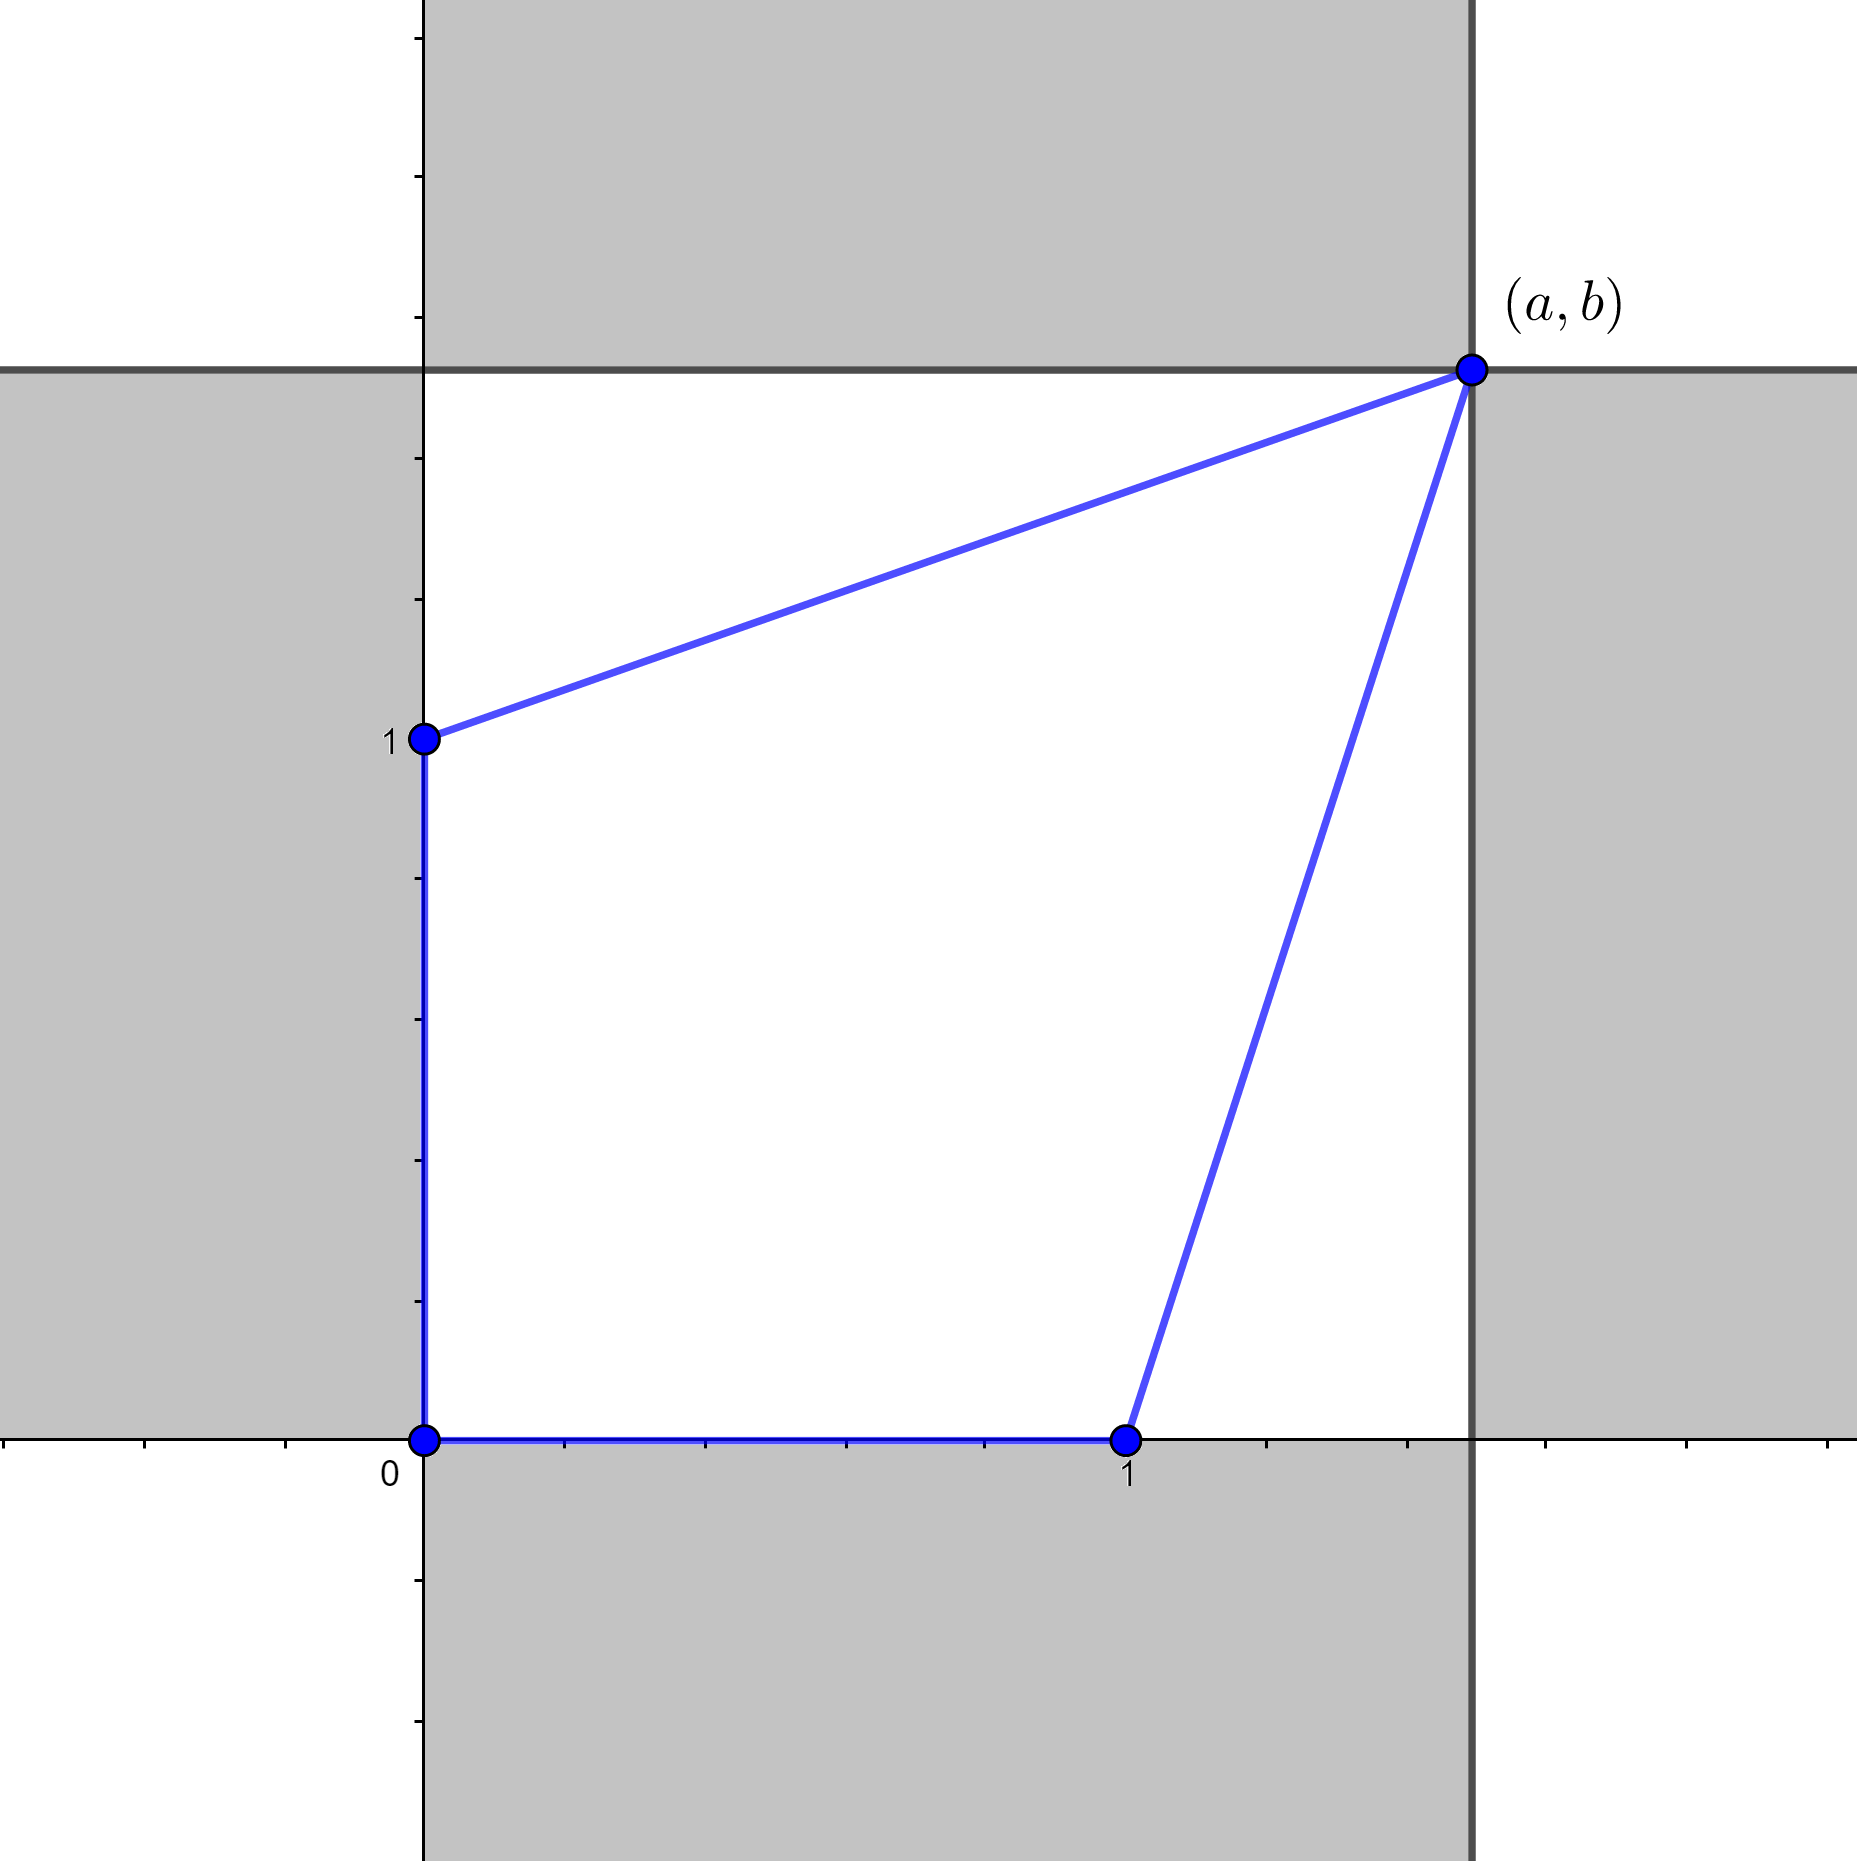
\includegraphics[width=0.35\linewidth]{pic23}
\end{figure}